% =====================================================================
%  Capítulo 5 — Ejercicios de observación
% =====================================================================
\chapter{Ejercicios de observación}
\citacap{Usted ve, pero no observa. La distinción es evidente.}{Sherlock Holmes, en Arthur Conan Doyle}

Permanentemente pasamos por diversos estados de vulnerabilidad: somos más o menos propensas a ser consideradas víctimas. El delincuente común va a elegir al objetivo menos complicado, y va a preferir a quien perciba como menos apta para defenderse por cuestión de edad, salud, distracción o descuido (llevar el bolso colgando a la espalda, el móvil en la mano absorbiendo toda la atención, la mano con reloj en la ventanilla del coche).

\textbf{Primer ejercicio:} dedica unos momentos al andar a ponerte en el rol de alguien que busca una víctima, y estudia a las demás personas para saber a quiénes y por qué \enquote{elegirías}. Observa qué factores transmiten vulnerabilidad y cuáles hacen descartar a otras personas.

\textbf{Segundo ejercicio:} también en la calle, toma consciencia de las personas que te rodean y determina su actividad: si van camino del trabajo o merodean; si algunas están solas pero parecen comunicarse visualmente con otras. Realiza detenciones periódicas ante escaparates y, con una mirada rápida, percibe si alguien hace tu mismo camino.

\textbf{Tercer ejercicio:} al entrar en cualquier local (bar, tienda, vagón), localiza en tres segundos las salidas y a las personas presentes. Al llegar a tu portal o coche, ten las llaves ya en la mano y mira alrededor antes de abrir.

El objetivo no es andar por la calle como una paranoica, sino que, al realizar todo esto a modo de juego, desarrollaremos gradualmente la observación y la capacidad de estar preparadas de forma natural, fijándose estos hábitos sin que nos demos cuenta.

\newpage

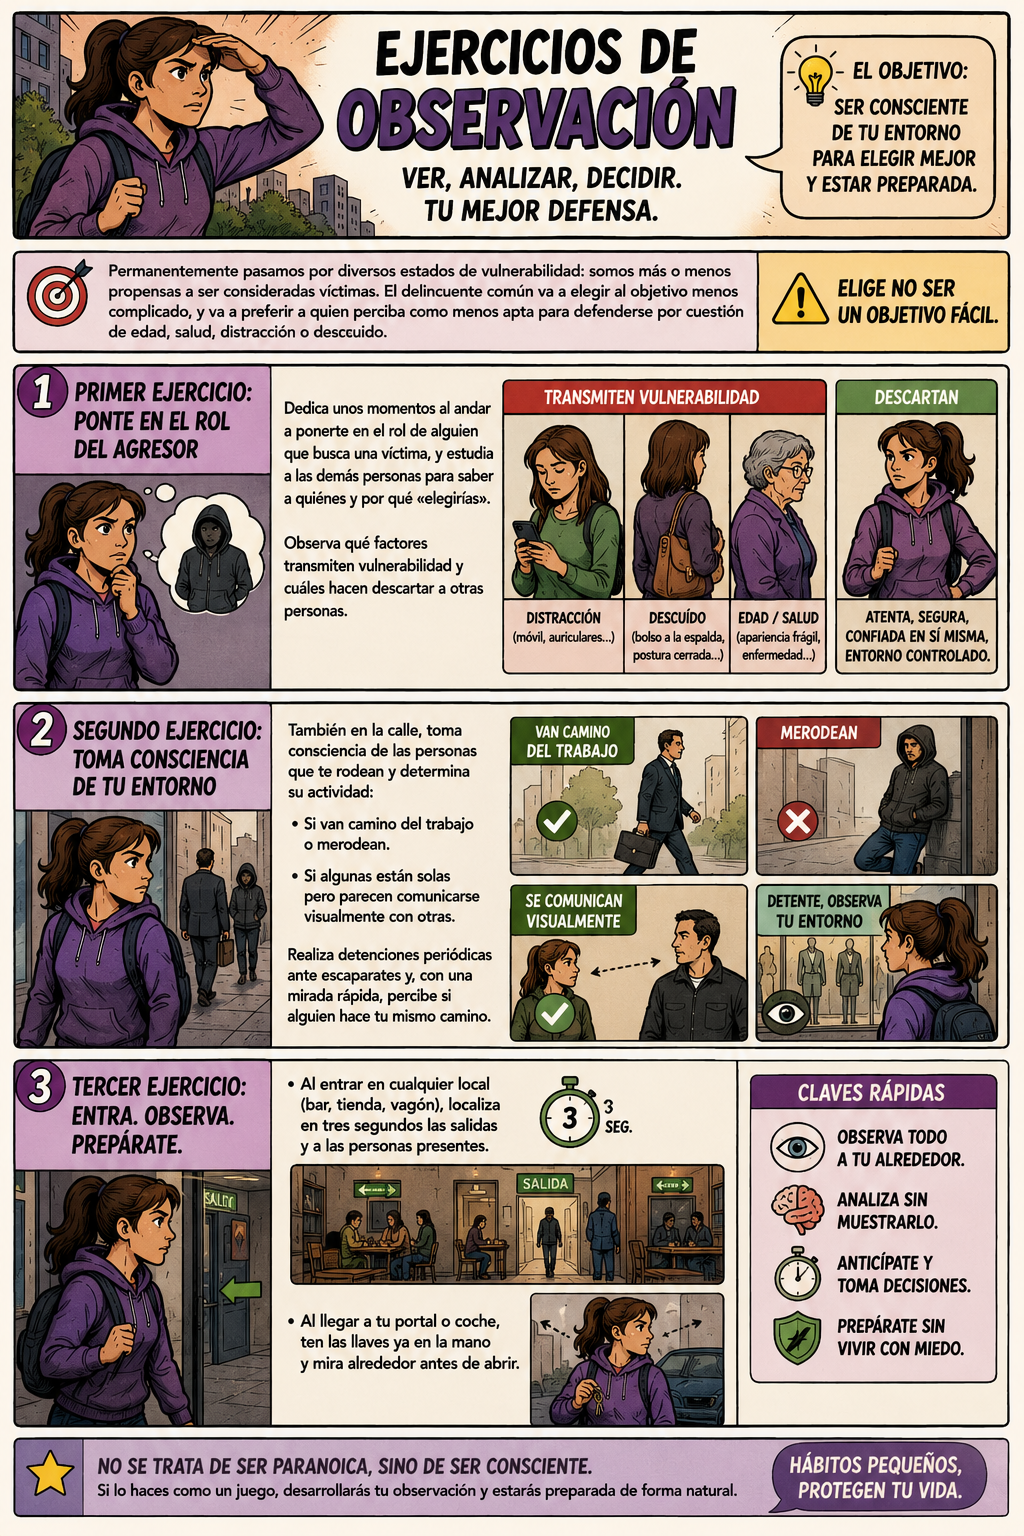
\includegraphics[width=\linewidth]{figures/observacion.png}
